%
% file: localoperator.tex
% author: Victor Brena
% description: Briefly describes properties of the local operator.
%

\chapter{Function Failure Identification and Propagation}
\label{app:app04}

\initial{S}everal initiating events are considered, and the propagation of the failures is computed using FFIP methodology. The loss of the function \textit{Signal - Sense - Measure} linked to the \textit{Energy - Radioactive} flow is propagated on figure~\ref{fig:ffip1}. This is equivalent to the loss of neutron detectors in a RBD. Next, the loss of the function {Channel - Guide - Rotate}, which connect the flow \textit{Material - Gas} with \textit{Energy - Mechanical} is propagated on figure~\ref{fig:ffip2}. This is equivalent to the loss of the turbines in a RBD. Furthermore, the loss of the function \textit{Convert - Convert} converting vapor flow to liquid flow is propagated on figure~\ref{fig:ffip3}. This is equivalent to the loss of the condensers in a RBD.

Two critical functions are defined. These functions are the one that are critical to the system reliability (electricity generation) and the system risks (preventing a core meltdown).

\begin{figure}[t]
\centering
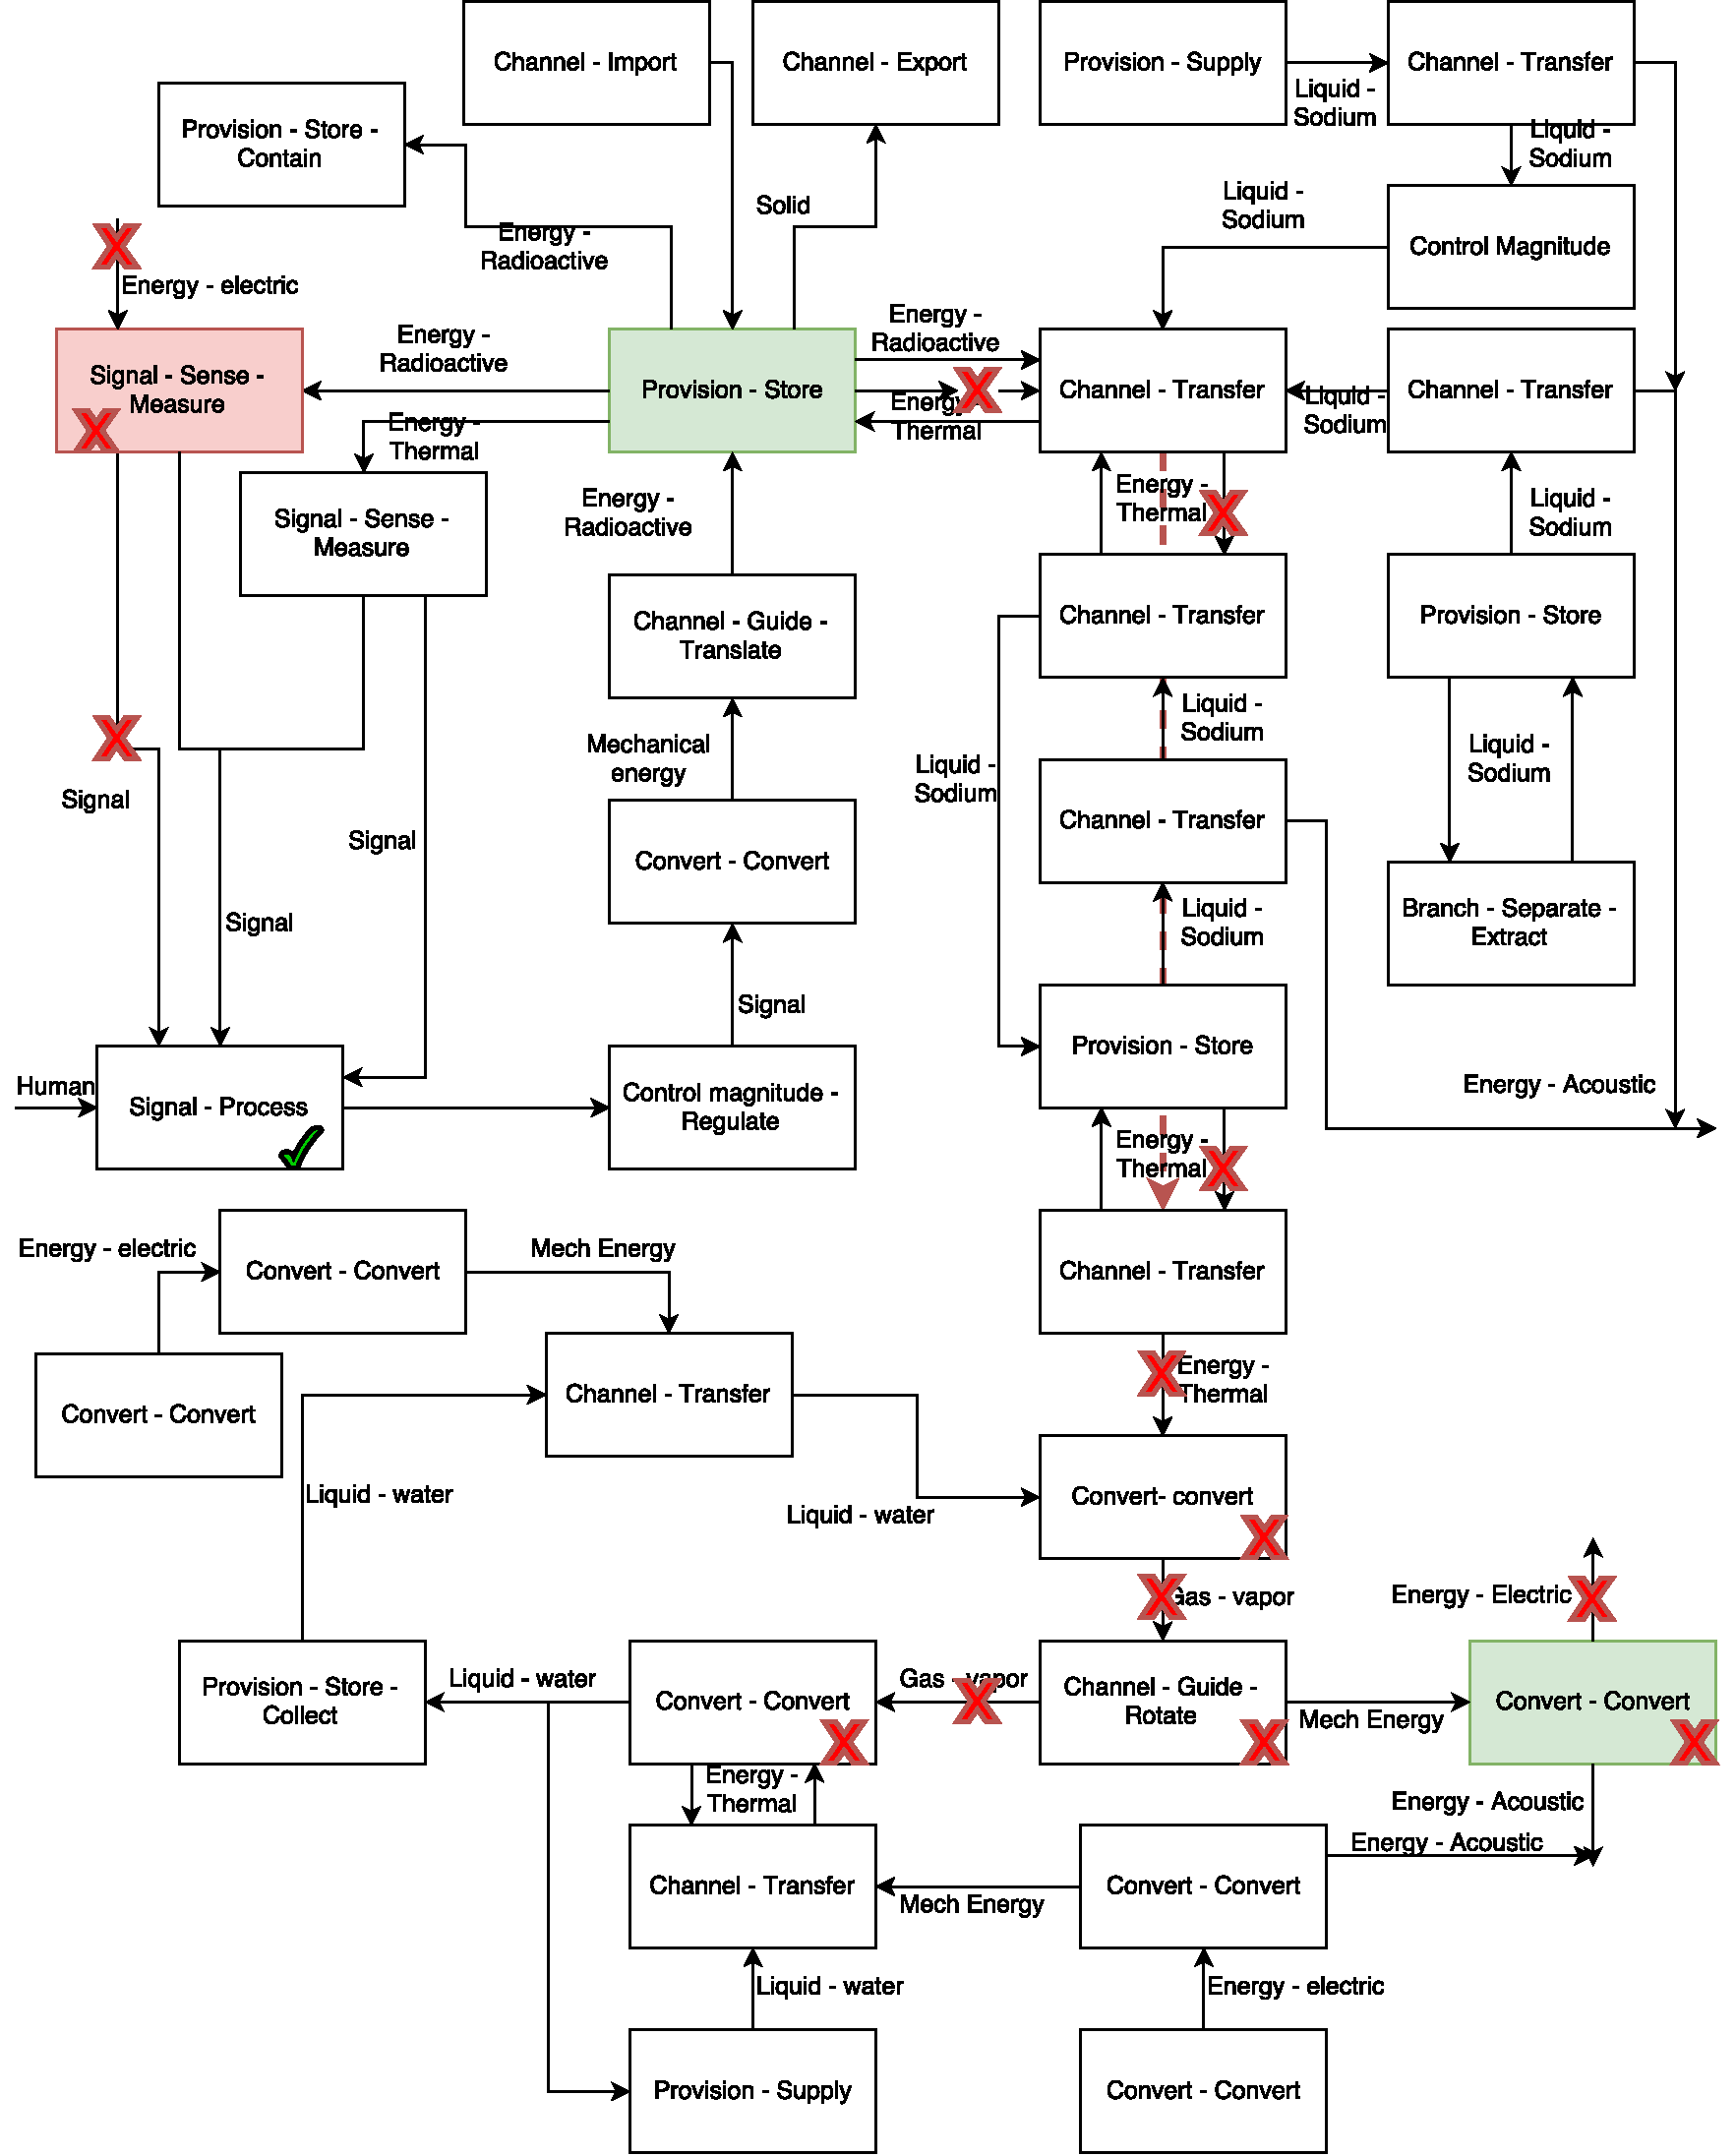
\includegraphics[scale=.55]{fig0d/FFIP_1}
\caption{FFIP - Initiating event: Loss of signal for the neutron detectors.}
\label{fig:ffip1}
\end{figure}



\begin{algorithm}
\caption{FFIP pseudocode - Function 1}\label{alg:ffip1}
\begin{algorithmic}[1]
\Procedure{Signal - Sense - Measure}{}
\Require {\textit{Energy - Electrical}, \textit{Energy - Radioactive}}
\Ensure {\textit{Signal}}
\If {$\textit{Energy - Electrical}_{in} = 0$} \Return procedure failed
\ElsIf {$\textit{Energy - Radioactive}_{in} > \max(\text{range})$} \Return procedure failed
\ElsIf {$\textit{Energy - Radioactive}_{in} < \min(\text{range})$} \Return procedure failed
\ElsIf {$\textit{Signal}_{out} = 0$} \Return procedure failed
\Else{} \Return procedure operative
\EndIf
\EndProcedure
\end{algorithmic}
\end{algorithm}


\begin{algorithm}
\caption{FFIP pseudocode - Function 2}\label{alg:ffip2}
\begin{algorithmic}[1]
\Procedure{Signal - Process}{}
\Require {\textit{Material - Human}, \textit{Energy - Electrical}, \textit{Signal}}
\Ensure {\textit{Signal - Control}}
\If {$\textit{Material - Human}_{in} = 0$ and $\textit{Energy - Electrical}_{in} = 0$} \Return procedure failed
\ElsIf {$\textit{Material - Human}_{in} = 0$ and $\textit{Signal}_{in} = 0$} \Return procedure failed
\ElsIf {$\textit{Signal - Control}_{out} = 0$} \Return procedure failed
\Else{} \Return procedure operative
\EndIf
\EndProcedure
\end{algorithmic}
\end{algorithm}


\begin{algorithm}
\caption{FFIP pseudocode - Function 3}\label{alg:ffip3}
\begin{algorithmic}[1]
\Procedure{Control Magnitude - Regulate}{}
\Require {\textit{Signal - Control}, \textit{Energy - Electrical}}
\Ensure {\textit{Signal - Control}}
\If {not $\textit{Signal - Control}_{in}$} \Return procedure SCRAM
\ElsIf {$\textit{Signal - Control}_{in} = 0$ and $\textit{Signal - Control}_{out} != 0$} \Return procedure failed
\ElsIf {$\textit{Signal - Control}_{in} = \pm 1$ and $\textit{Signal - Control}_{out}\ in\ [0, \mp \textit{Signal - Control}_{in}$]} \Return procedure failed
\ElsIf {$\textit{Signal - Control}_{in}$ and $\textit{Energy - Electrical}_{in} = 0$} \Return procedure failed
\Else{} \Return procedure operative
\EndIf
\EndProcedure
\end{algorithmic}
\end{algorithm}


\begin{algorithm}
\caption{FFIP pseudocode - Function 4}\label{alg:ffip4}
\begin{algorithmic}[1]
\Procedure{Convert - Convert}{}
\Require {\textit{Signal - Control}, \textit{Energy - Electrical}}
\Ensure {\textit{Energy - Mechanical}}
\If {not $\textit{Signal - Control}_{in}$} \Return procedure SCRAM
\ElsIf {$\textit{Signal - Control}_{in}$ and $\textit{Energy - Electrical}_{in} = 0$} \Return procedure failed
\ElsIf {$\textit{Signal - Control}_{in}$ and $\textit{Energy - Mechanical}_{out} = 0$} \Return procedure failed
\Else{} \Return procedure operative
\EndIf
\EndProcedure
\end{algorithmic}
\end{algorithm}


\begin{algorithm}
\caption{FFIP pseudocode - Function 5}\label{alg:ffip5}
\begin{algorithmic}[1]
\Procedure{Channel - Guide - Translate}{}
\Require {\textit{Material - Mixture - Solid-Solid}, \textit{Energy - Mechanical}}
\Ensure {\textit{Energy - Radioactive}}
\If {$\textit{Energy - Radioactive}_{out}$ not change} \Return procedure failed
\Else{} \Return procedure operative
\EndIf
\EndProcedure
\end{algorithmic}
\end{algorithm}


\begin{figure}[t]
\centering
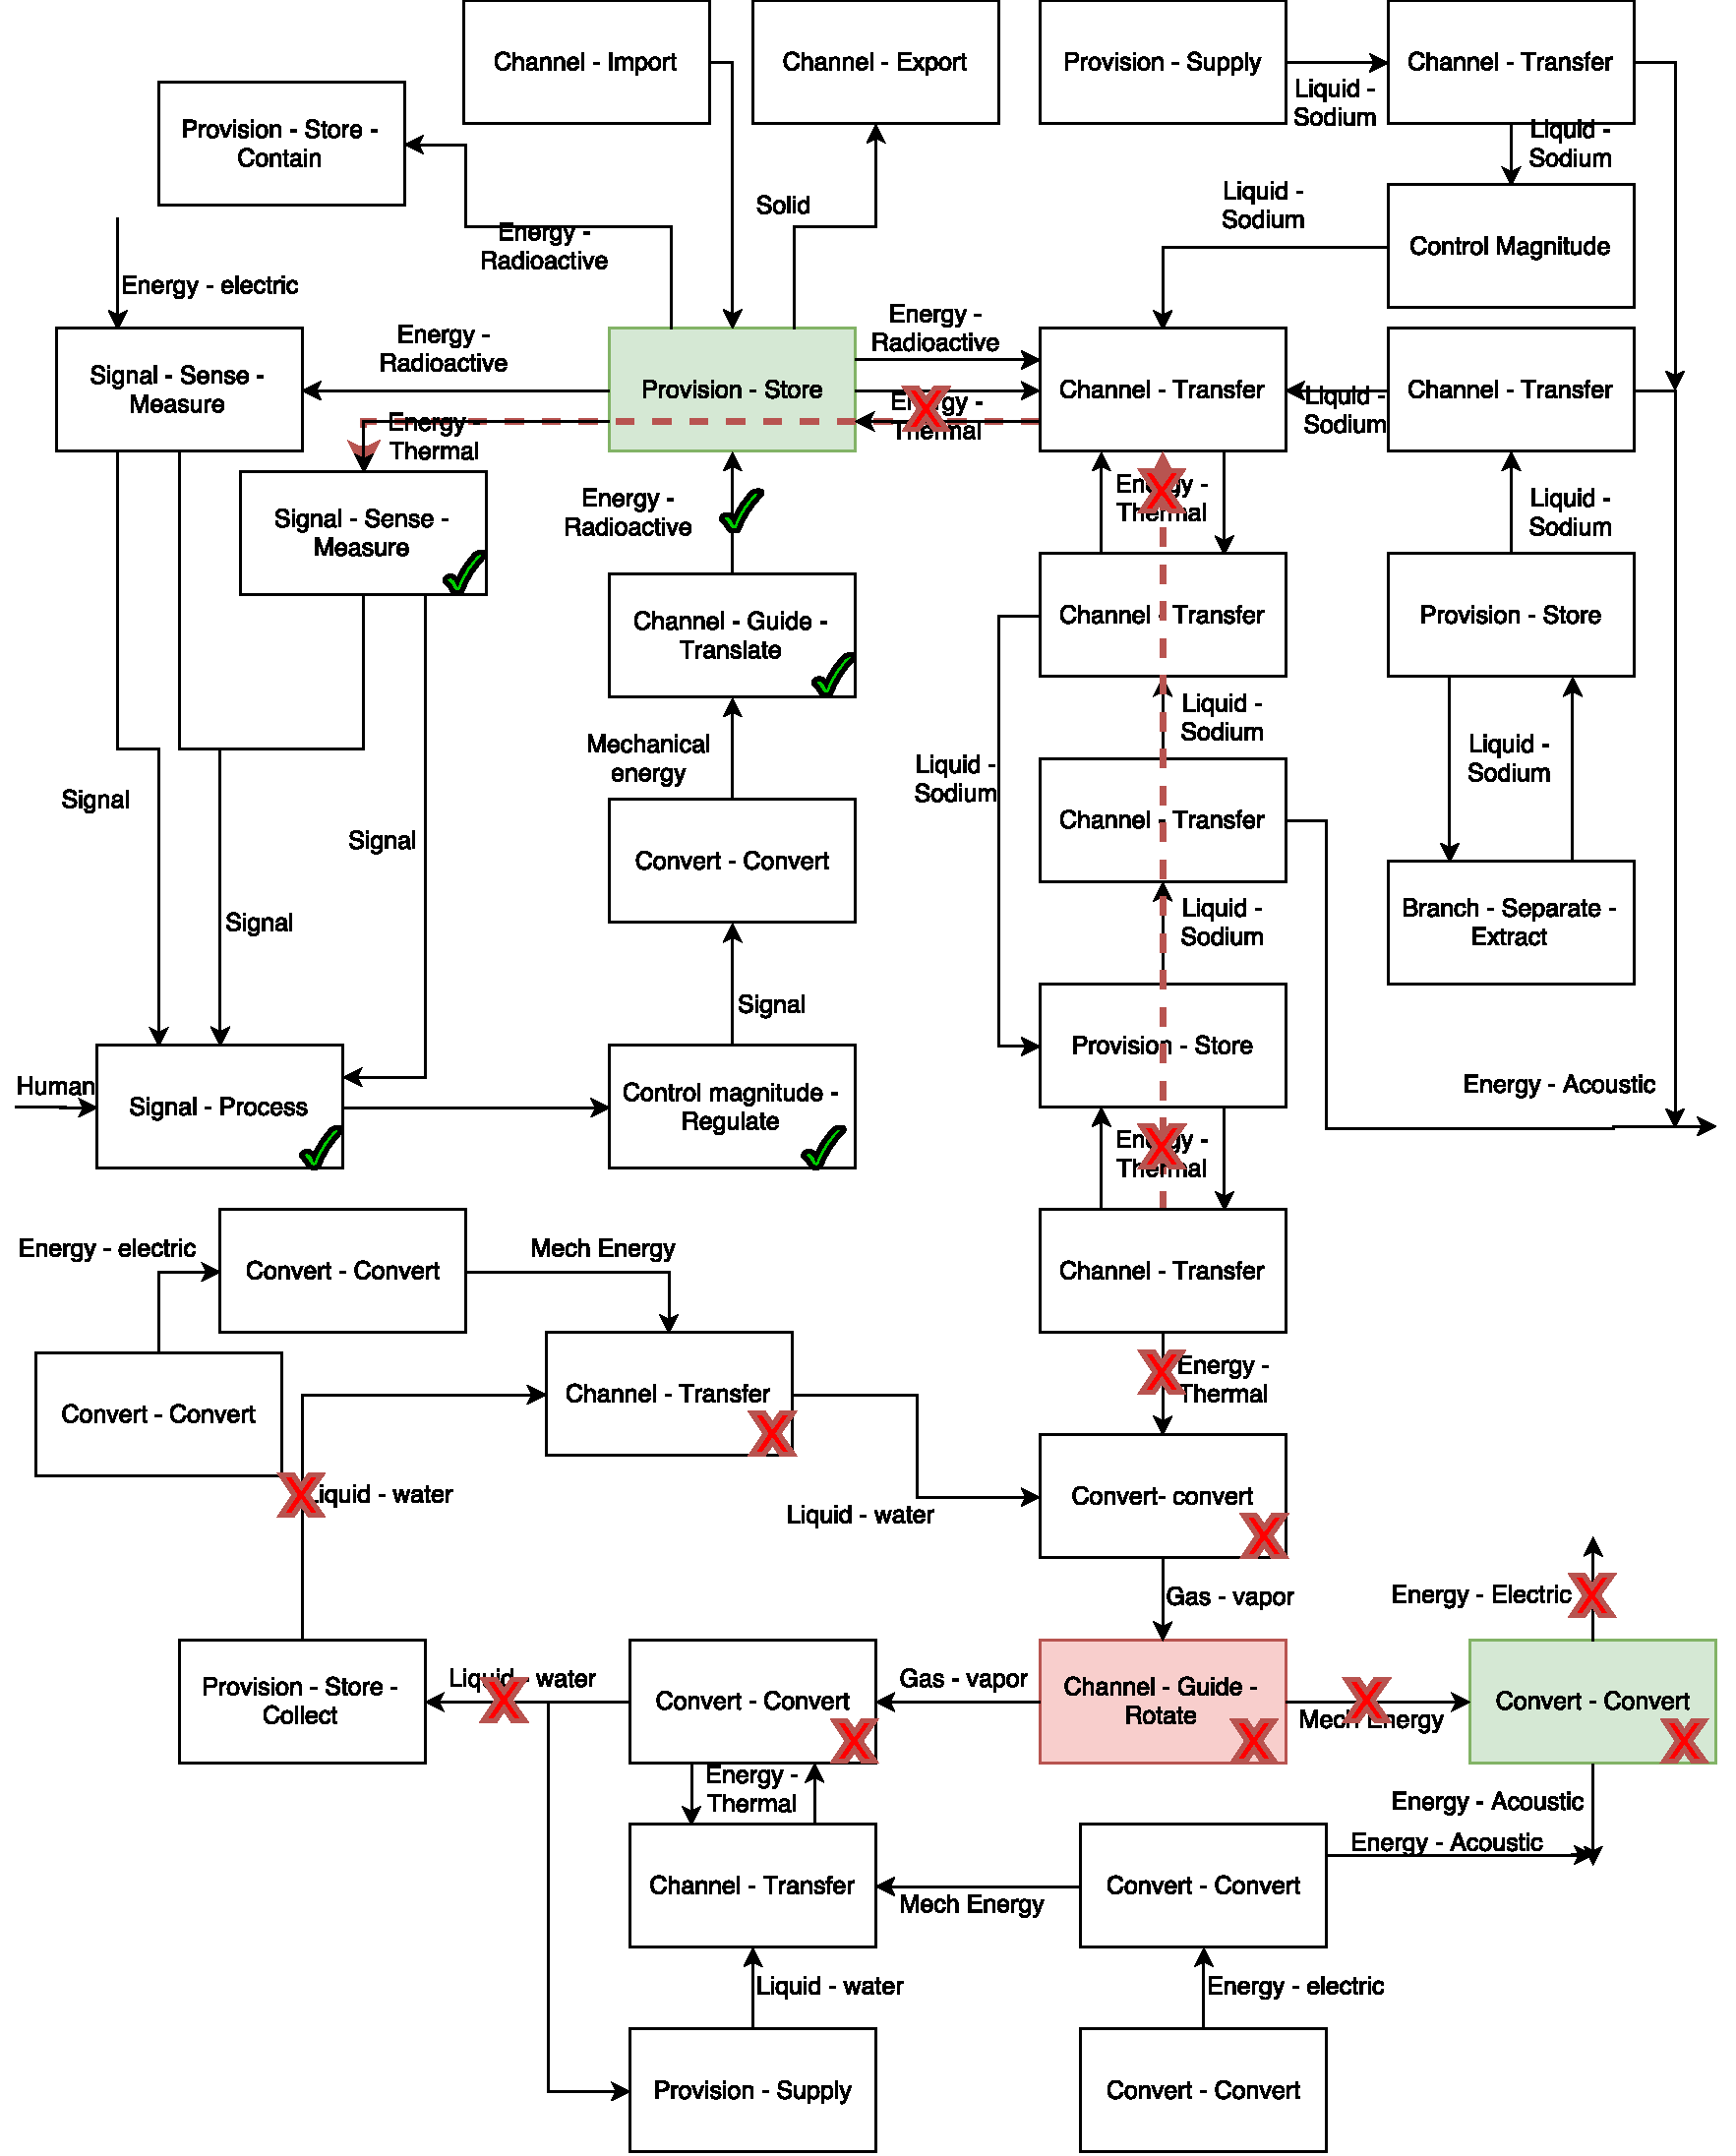
\includegraphics[scale=.55]{fig0d/FFIP_2}
\caption{FFIP - Initiating event: Loss of turbines.}
\label{fig:ffip2}
\end{figure}

\begin{figure}[t]
\centering
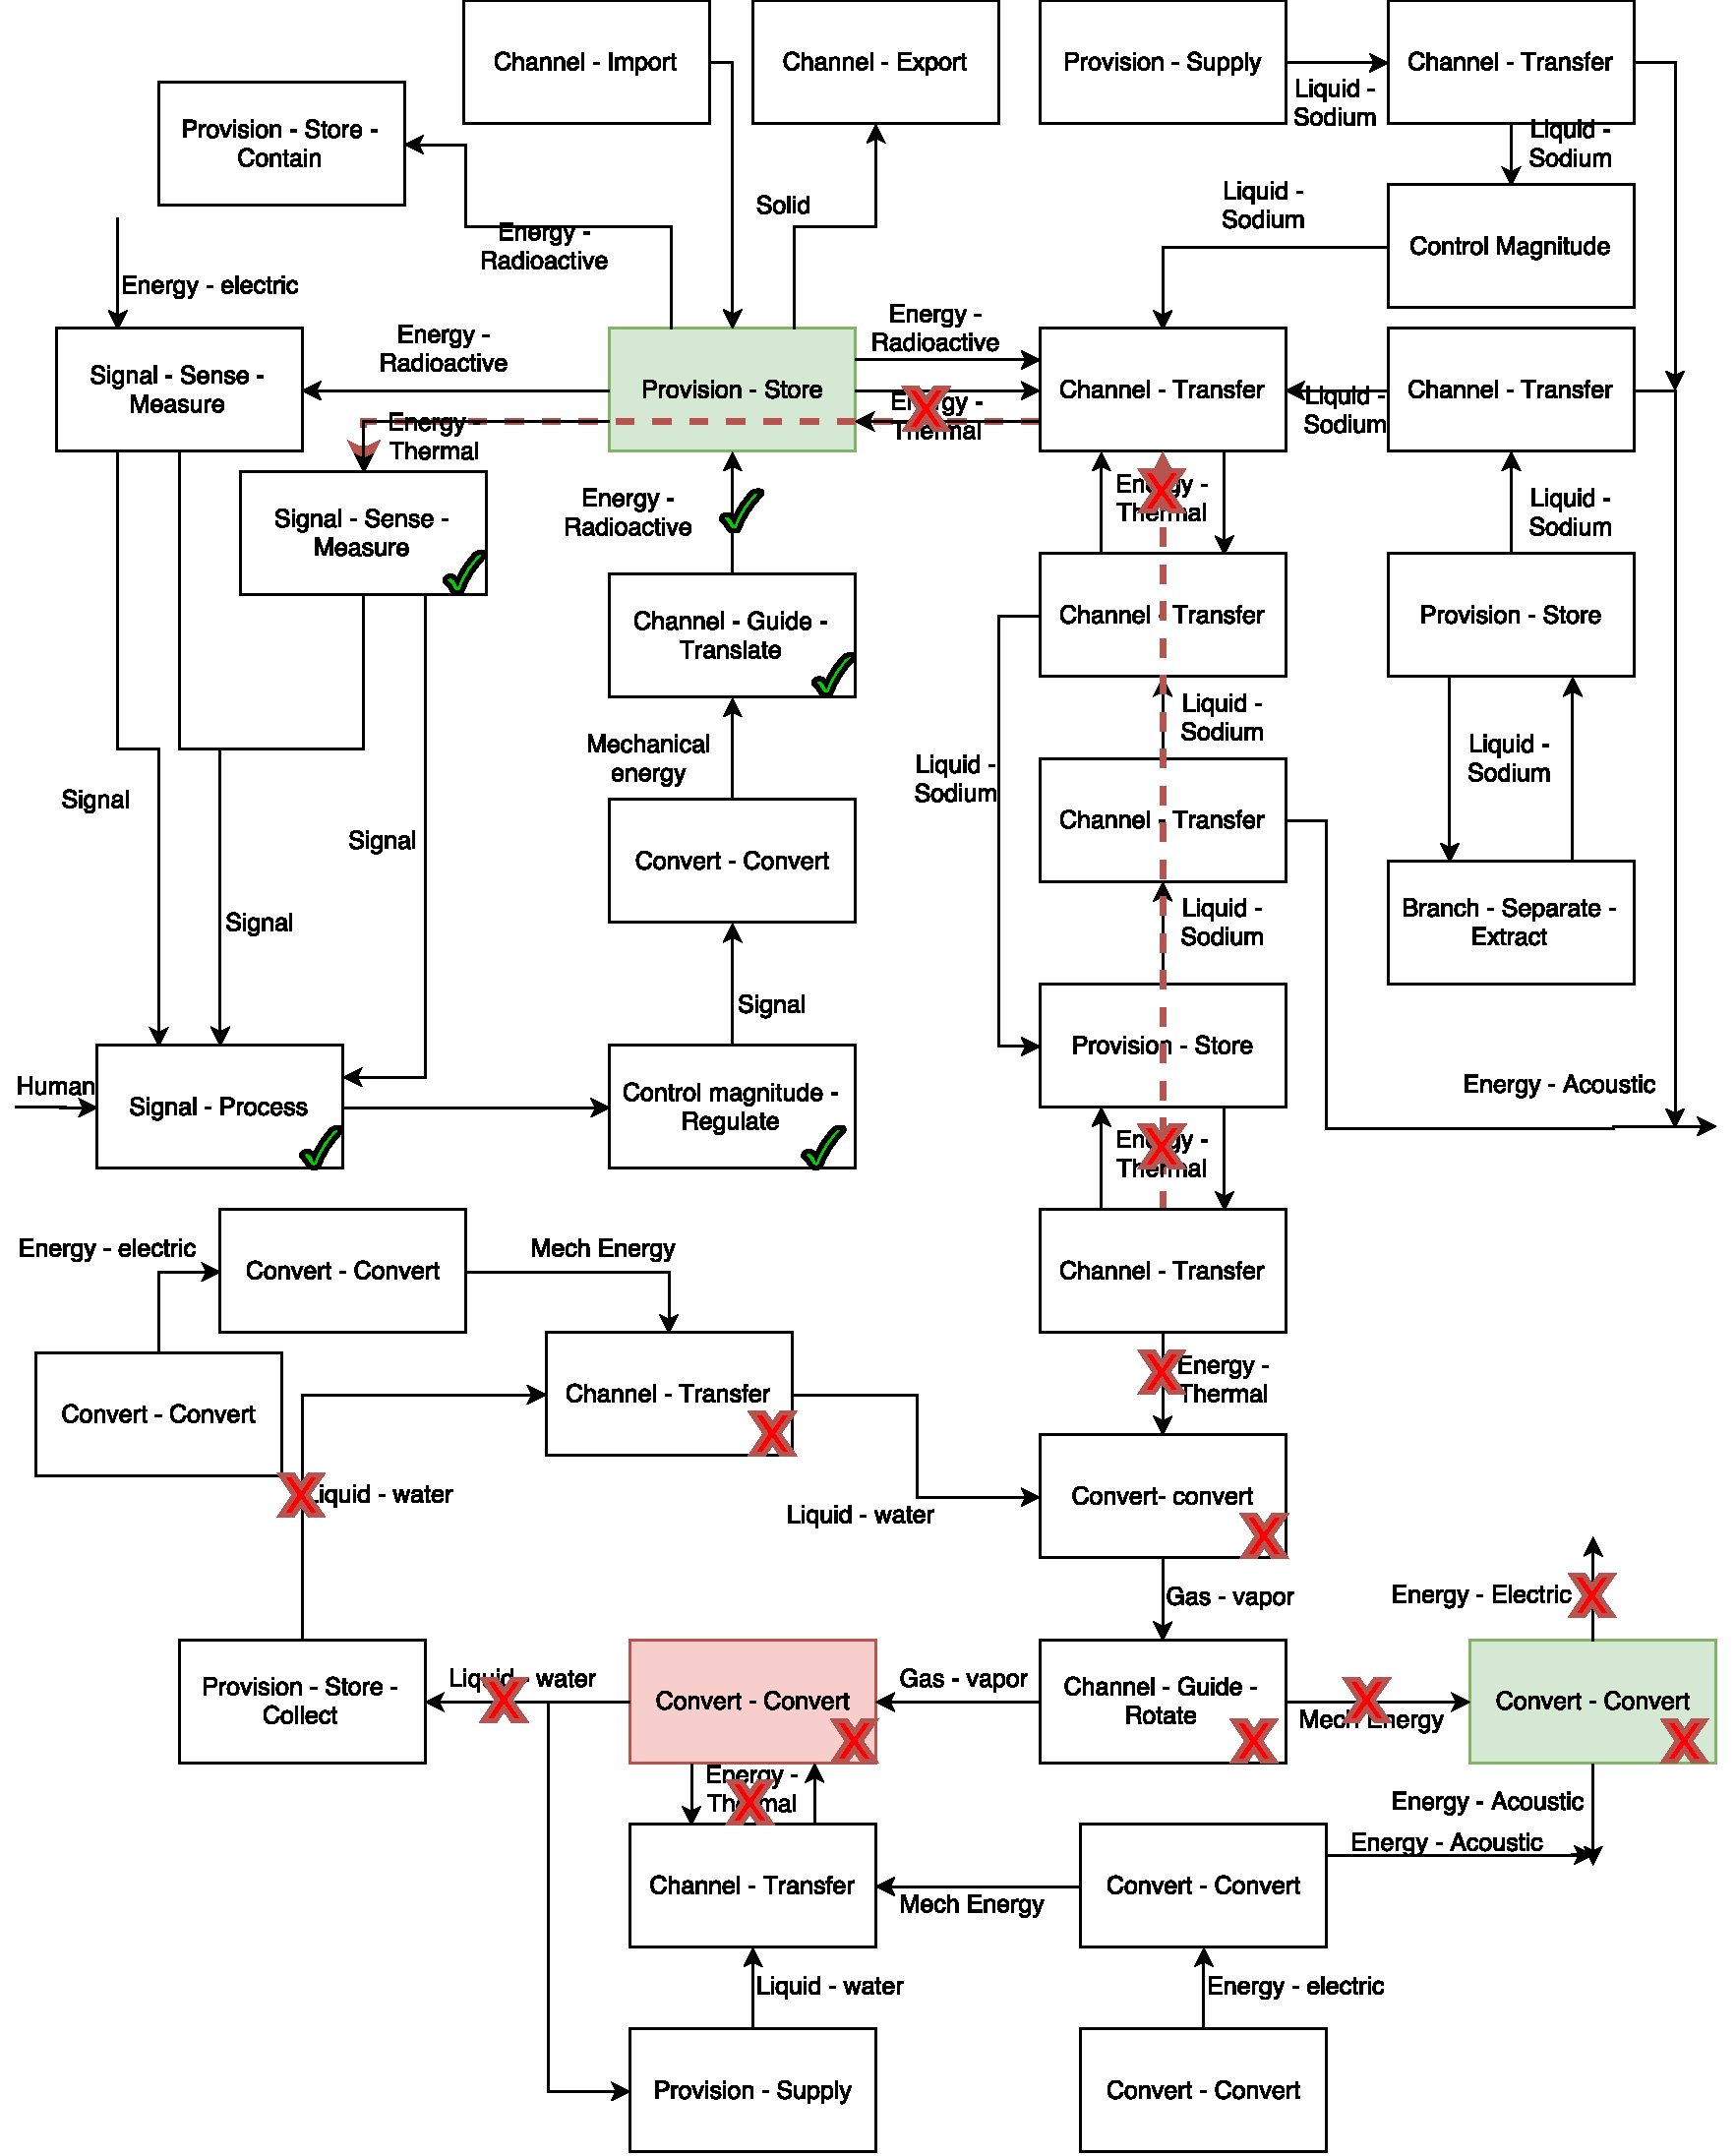
\includegraphics[scale=.55]{fig0d/FFIP_3}
\caption{FFIP - Initiating event: Loss of condensers.}
\label{fig:ffip3}
\end{figure}

\begin{figure}[t]
\centering
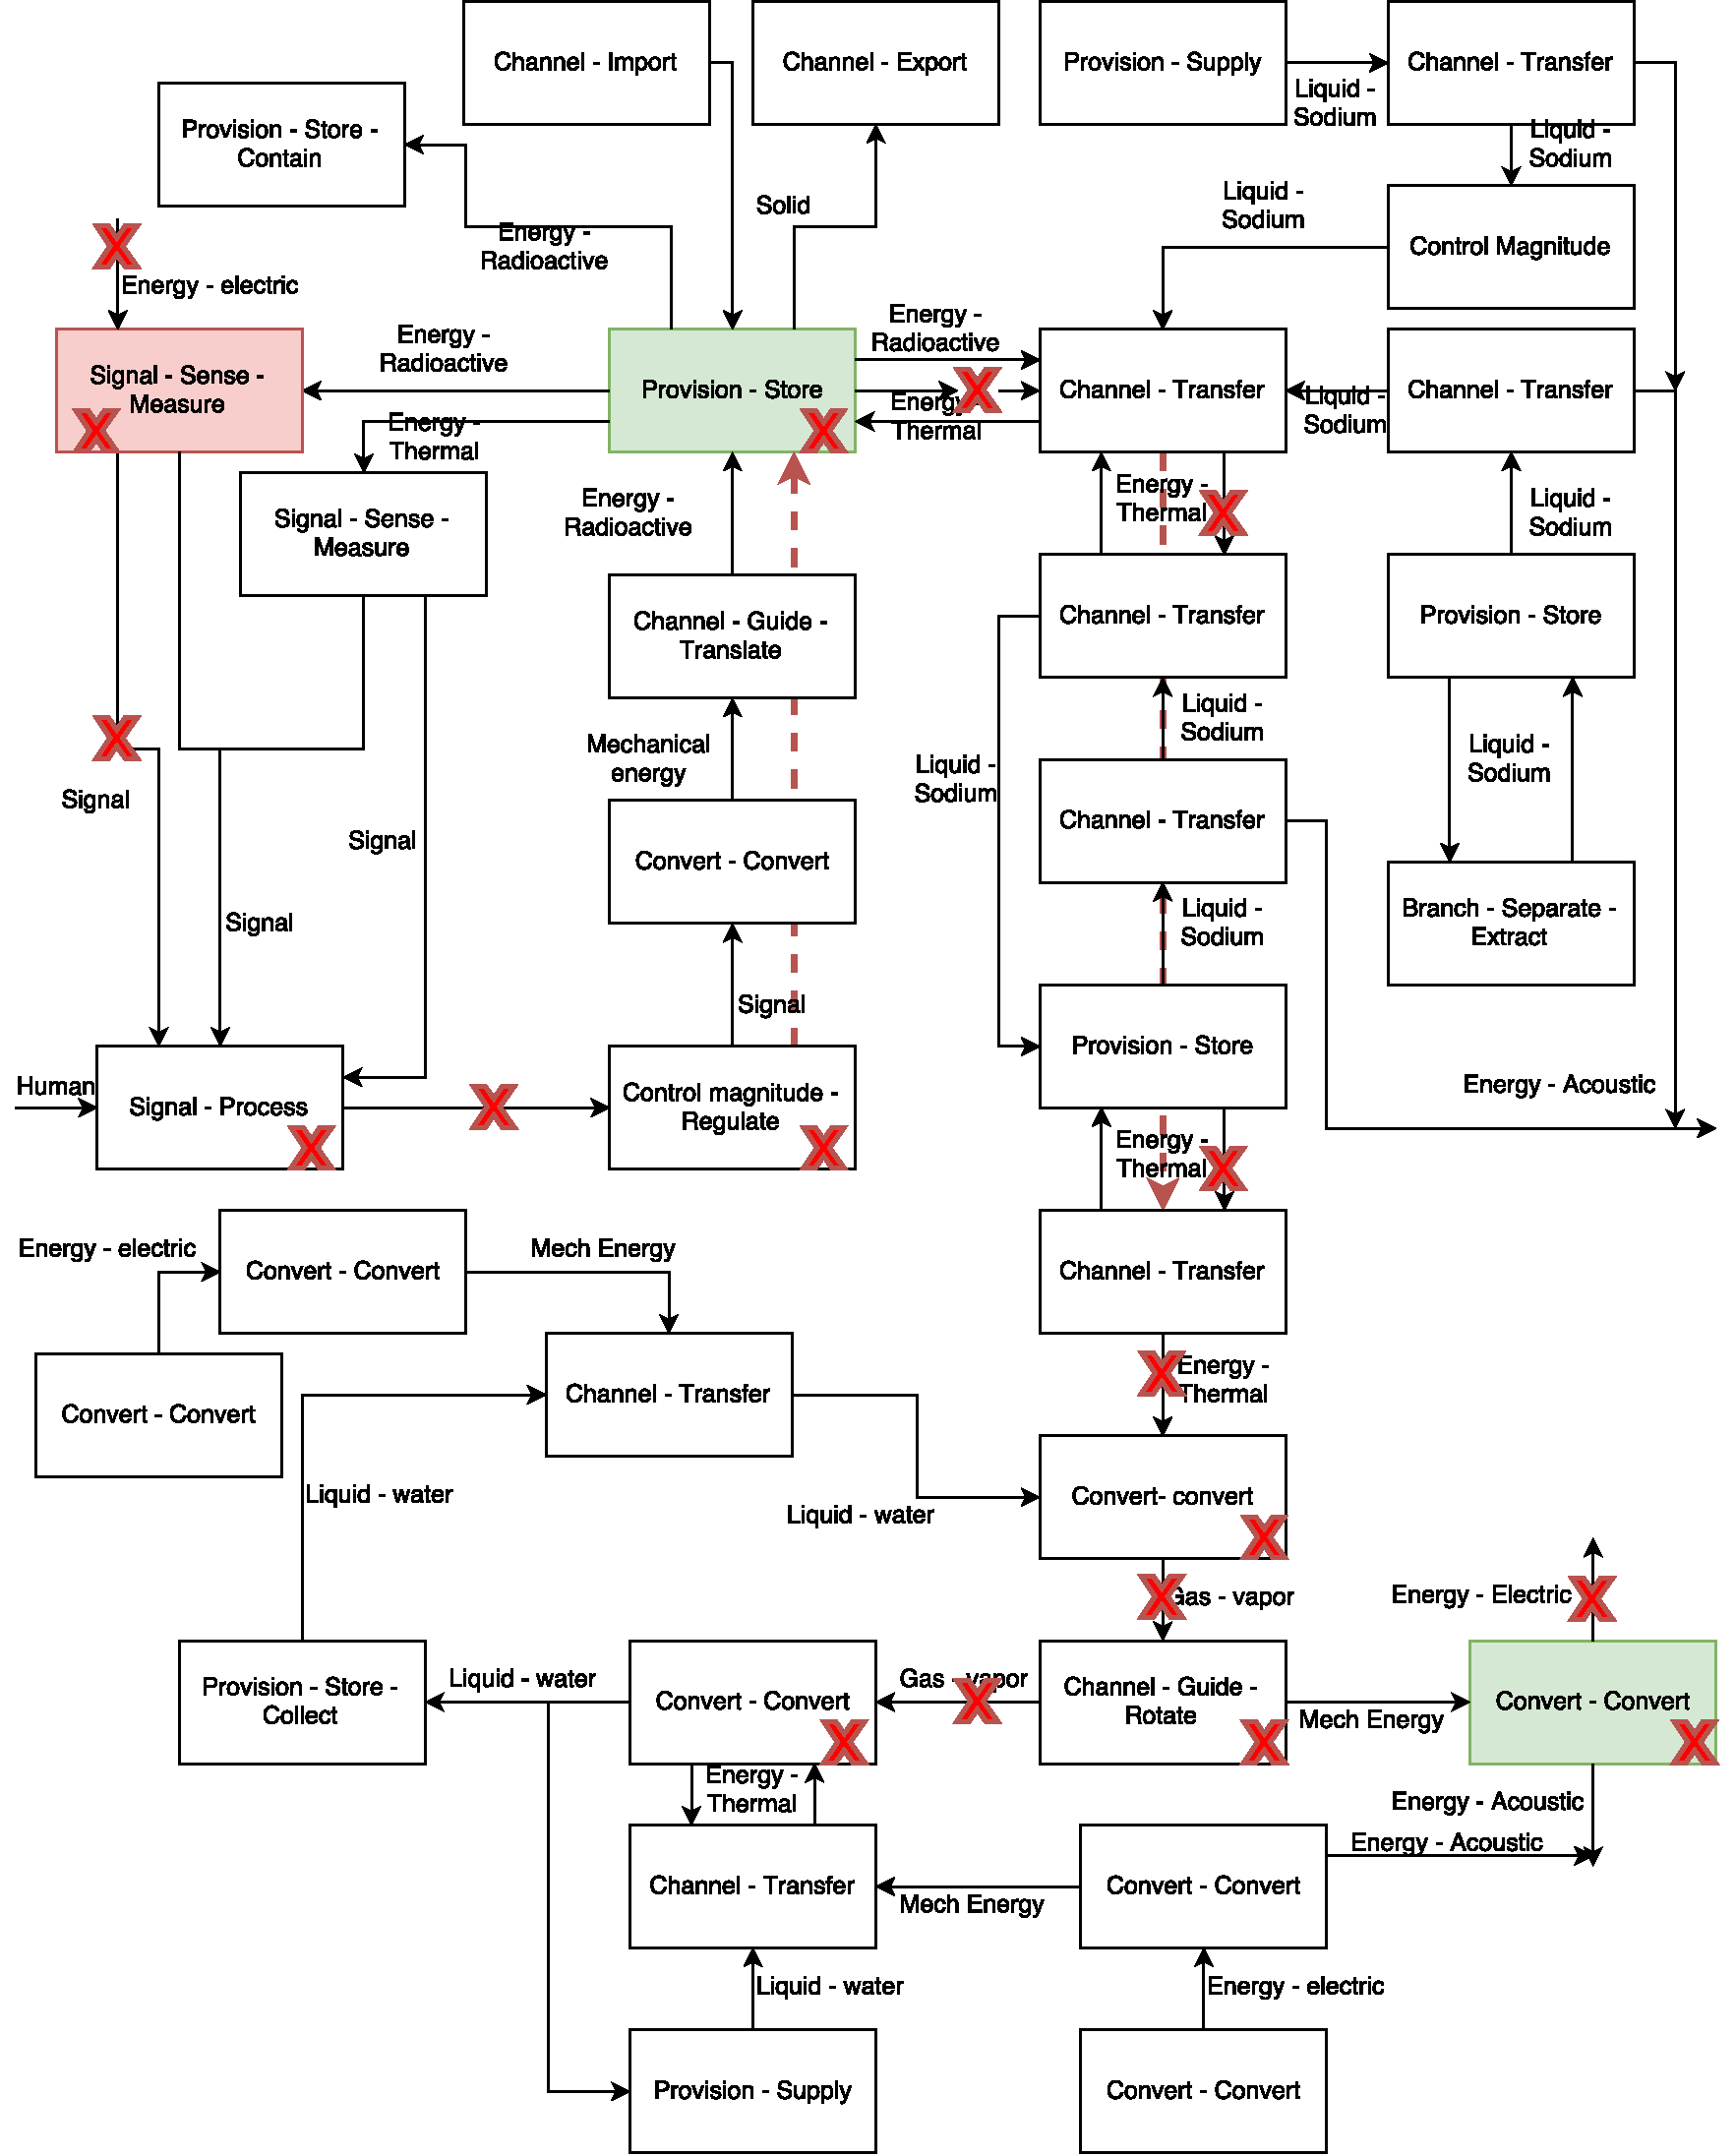
\includegraphics[scale=.55]{fig0d/FFIP_4}
\caption{FFIP - Initiating event: Loss of signal for the neutron detectors - Alternative scenario}
\label{fig:ffip4}
\end{figure}


\
